\documentclass[10pt]{beamer}
\usetheme{Warsaw}
\usepackage[utf8]{inputenc}
\usepackage[french]{babel}
%\usepackage[T1]{fontenc}
\usepackage{amsmath}
\usepackage{amsfonts}
\usepackage{amssymb}
\usepackage{graphicx}
\usepackage{lmodern}
\usepackage{listings}%Code source
\usepackage{color}
\usepackage{animate}
\usepackage{verbatim}
\usepackage{float}
\usepackage{array,multirow,rotating,hhline,subfig}
\usepackage[
    type={CC},    
    modifier={by-nc-sa},
    version={3.0},
]{doclicense}

\author{Jean-Mathieu Chantrein}
\title{Fondements de la technologie de conteneurisations docker}
\titlegraphic{\includegraphics[scale=0.68]{img/docker-logo}}
%\setbeamercovered{transparent} 
\setbeamertemplate{navigation symbols}{} 
%\logo{\includegraphics[scale=0.2]{img/logo} \newline \v\includegraphics[scale=0.2]{img/by-nc-sa1.png}}
\logo{\vspace{-0.47cm}\includegraphics[scale=0.15]{img/logos}}

\institute{LERIA} 
%\date{} 


%\setbeamercovered{invisible}
\setbeamercovered{dynamic}

\setbeamertemplate{navigation symbols}{}
\addtobeamertemplate{footline}{\hfill\insertframenumber/\inserttotalframenumber\hspace{2em}\null}

\setbeamersize{text margin left=10px}
\setbeamersize{text margin right=10px}

%Configuration listing
\definecolor{mygreen}{rgb}{0,0.6,0}
\definecolor{mygray}{rgb}{0.5,0.5,0.5}
\definecolor{mymauve}{rgb}{0.58,0,0.82}

% Debut Ecriture et la coloration syntaxique de code
\usepackage{listings} 
\lstdefinestyle{customcpp}{
%belowcaptionskip=0\baselineskip,
%escapeinside={(?}{?)},
basicstyle=\scriptsize\ttfamily,
%extendedchars=true,
%breaklines=true,
%frame=L,
%xleftmargin=\parindent,
language=C++,
showstringspaces=false,
%basicstyle=\footnotesize\ttfamily,
keywordstyle=\bfseries\color{green!40!black},
commentstyle=\color{purple!40!black},
identifierstyle=\color{blue},
stringstyle=\color{orange},
tabsize=4,
otherkeywords={signals,SIGNAL,slots,SLOT,Q_OBJECT}
}

\lstset{escapechar=@,style=customcpp}

\lstset{literate=
{á}{{\'a}}1 {é}{{\'e}}1 {í}{{\'i}}1 {ó}{{\'o}}1 {ú}{{\'u}}1
{Á}{{\'A}}1 {É}{{\'E}}1 {Í}{{\'I}}1 {Ó}{{\'O}}1 {Ú}{{\'U}}1
{à}{{\`a}}1 {è}{{\`e}}1 {ì}{{\`i}}1 {ò}{{\`o}}1 {ù}{{\`u}}1
{À}{{\`A}}1 {È}{{\'E}}1 {Ì}{{\`I}}1 {Ò}{{\`O}}1 {Ù}{{\`U}}1
{ä}{{\"a}}1 {ë}{{\"e}}1 {ï}{{\"i}}1 {ö}{{\"o}}1 {ü}{{\"u}}1
{Ä}{{\"A}}1 {Ë}{{\"E}}1 {Ï}{{\"I}}1 {Ö}{{\"O}}1 {Ü}{{\"U}}1
{â}{{\^a}}1 {ê}{{\^e}}1 {î}{{\^i}}1 {ô}{{\^o}}1 {û}{{\^u}}1
{Â}{{\^A}}1 {Ê}{{\^E}}1 {Î}{{\^I}}1 {Ô}{{\^O}}1 {Û}{{\^U}}1
{œ}{{\oe}}1 {Œ}{{\OE}}1 {æ}{{\ae}}1 {Æ}{{\AE}}1 {ß}{{\ss}}1
{ű}{{\H{u}}}1 {Ű}{{\H{U}}}1 {ő}{{\H{o}}}1 {Ő}{{\H{O}}}1
{ç}{{\c c}}1 {Ç}{{\c C}}1 {ø}{{\o}}1 {å}{{\r a}}1 {Å}{{\r A}}1
{€}{{\EUR}}1 {£}{{\pounds}}1 {'}{{'}}1
}

% Fin Ecriture et la coloration syntaxique de code


%\lstset{ 
%backgroundcolor=\color{white},   % choose the background color; you must add \usepackage{color} or \usepackage{xcolor}; should come as last argument
%basicstyle=\footnotesize,        % the size of the fonts that are used for the code
%breakatwhitespace=false,         % sets if automatic breaks should only happen at whitespace
%breaklines=true,                 % sets automatic line breaking
%captionpos=b,                    % sets the caption-position to bottom
%commentstyle=\color{mygreen},    % comment style
%deletekeywords={...},            % if you want to delete keywords from the given language
%escapeinside={\%*}{*)},          % if you want to add LaTeX within your code
%extendedchars=true,              % lets you use non-ASCII characters; for 8-bits encodings only, does not work with UTF-8
%frame=single,	                   % adds a frame around the code
%keepspaces=true,                 % keeps spaces in text, useful for keeping indentation of code (possibly needs columns=flexible)
%keywordstyle=\color{blue},       % keyword style
%language=bash,                 % the language of the code
%morekeywords={*,...},            % if you want to add more keywords to the set
%numbers=left,                    % where to put the line-numbers; possible values are (none, left, right)
%numbersep=5pt,                   % how far the line-numbers are from the code
%numberstyle=\tiny\color{mygray}, % the style that is used for the line-numbers
%rulecolor=\color{black},         % if not set, the frame-color may be changed on line-breaks within not-black text (e.g. comments (green here))
%showspaces=false,                % show spaces everywhere adding particular underscores; it overrides 'showstringspaces'
%showstringspaces=false,          % underline spaces within strings only
%showtabs=false,                  % show tabs within strings adding particular underscores
%stepnumber=2,                    % the step between two line-numbers. If it's 1, each line will be numbered
%stringstyle=\color{mymauve},     % string literal style
%tabsize=2,	                   % sets default tabsize to 2 spaces
%title=\lstname                   % show the filename of files included with \lstinputlisting; also try caption instead of title
%}
%Fin Configuration listing


\newenvironment<>{shell}[1]{%
	\setbeamercolor{block title}{fg=white,bg=black}%
	\setbeamercolor{block body}{fg=white,bg=black}
	\begin{block}#2{\underline{Terminal:}}}{\normalsize \end{block}
}
\newenvironment<>{shellContainer}[1]{%
	\setbeamercolor{block title}{fg=white,bg=gray}%
	\setbeamercolor{block body}{fg=white,bg=gray}
	\vspace{-0.4cm}\begin{block}#2{\underline{Conteneur:}}}{\normalsize \end{block}
}
%\newenvironment<>{examplesecond}[1]{%
%	\setbeamercolor{block title}{fg=white,bg=blue!75!black}%
%	\begin{block}#2{#1}}{\end{block}
%}

\newcommand\prompt{\textcolor{green}{jmc@laptop}\textcolor{cyan}{ /home/jmc \$ }}
\newcommand\promptsshd{\textcolor{green}{jmc@laptop}\textcolor{cyan}{ /home/jmc/sshd \$ }}

\begin{document}

\AtBeginSubsection[]
{
	\begin{frame}{Plan}
	\tableofcontents[currentsection] %,hideallsubsections
	\end{frame}
}

%\AtBeginSubsection[]
%{
%	\begin{frame}
%	\begin{columns}[t]
%		\begin{column}{6cm}
%			\tableofcontents[sections={1-3},currentsection, currentsubsection]
%		\end{column}
%		\begin{column}{6cm}
%    		\tableofcontents[sections={4-7},currentsection,currentsubsection]
%		\end{column}
%	\end{columns}
%\end{frame}
%}

%\small


\begin{frame}
\titlepage

\end{frame}

\begin{frame}{Licence}
	\begin{block}{}
		\doclicenseThis
	\end{block}
\end{frame}

\begin{frame}{Plan}
	\tableofcontents
\end{frame}



\section{Introduction générale}
\subsection{Conteneur versus machine virtuelle}


\begin{frame}{Introduction}
	\begin{block}{}
		Dans cette section nous allons définir quelques notions qui nous permettront de mieux appréhender les principales différences qu'il y a entre une machine physique (réelle), une machine virtuelle et un conteneur. 
	\end{block}
\end{frame}


\begin{frame}{Au commencement il y avait ...}
	\begin{block}{... la machine physique: l'ordinateur (serveur, PC, Mac, ...)}
		\begin{itemize}
			\item Il est fabriqué principalement avec des composants électroniques
			\pause
			\item Il est programmable (on peut lui faire exécuter des programmes)
			\pause
			\item Il est très puissant pour effectuer des calculs binaires (mais il ne sait faire que ça)
			\pause
		\end{itemize}
	\end{block}
	\begin{block}{Système d'exploitation (Operating System, abrégé OS)}
		Un système d'exploitation est un programme qui a pour but : 
		\begin{itemize}
			\item d'assurer la communication entre des logiciels et les différents composants d'une machine (device (RAM, HDD, carte réseau, ...))
			\pause
			\item d'organiser/planifier l'exécution d'autres programmes

		\end{itemize}	
	\end{block}
\end{frame}


\begin{frame}{Ensuite, il y a eu la virtualisation ...}
	\begin{block}{... de machine (machine virtuelle, virtual machine, abrégé VM)}
		\begin{itemize}
			\item Une machine virtuelle est une machine émulée par un logiciel. 
			\pause
			\item Le logiciel d'émulation simule la présence de ressources matérielles telles que la mémoire, le(s) processeur(s), le(s) disque(s) dur. 
			\pause
			\item Le logiciel d'émulation est capable de simuler un ordinateur.
			\pause
			\item On appelle hyperviseur le logiciel ayant pour mission de gérer les VM (QEMU/KVM, HyperV, VMWare, VirtualBox, Xen, Proxmox, ...)
			\pause
			\item Il y a 2 types d'hyperviseur:
			\begin{itemize}
				\item type 1 (bare metal ou native) meilleure performance, l'hyperviseur est l'os (Ex: Xen, Qemu/KVM) (VM "aware")
				\item type 2 (hosted): Hyperviseur sur OS (Virtual Box) (VM "no aware")
			\end{itemize}
		\end{itemize}
	\end{block}
\end{frame}

\begin{frame}{Architecture simplifiée du modèle VM/hyperviseur}
	\begin{minipage}[b]{.49\linewidth}
		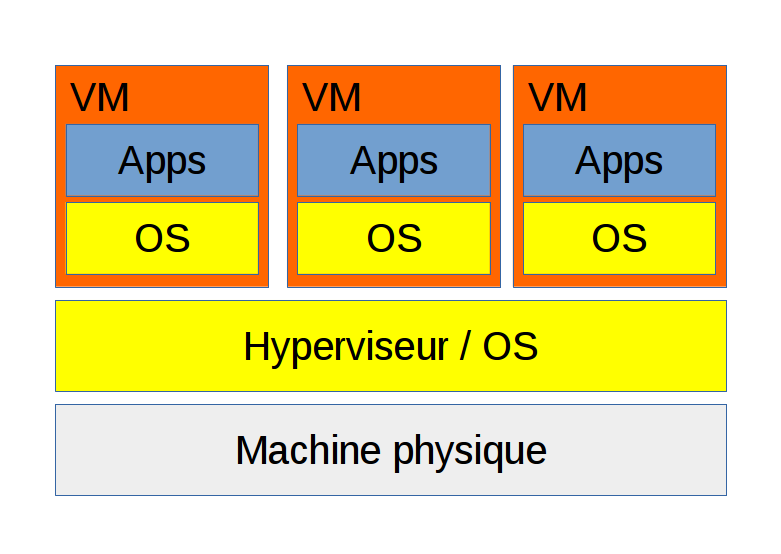
\includegraphics[width=\linewidth]{img/hyperviseur.png}
	\end{minipage}
	\hfill
	\begin{minipage}[b]{.49\textwidth}
		\begin{overprint}
			\only<2-6>{
				\begin{block}{Avantages}
					\begin{itemize}
						\item<2-> Portabilité des VM
						\item<3-> Isolation des applications
						\item<4-> Mutualisations des ressources
						\item<5-> Ressources à la demande
						\item<6-> Démarrage plus rapide qu'une machine réelle	
					\end{itemize}
				\end{block}
			}
			\only<7->{
				\begin{alertblock}{Inconvénients}
					\begin{itemize}
						\item<7-> Performance inférieure à une exécution native
						\item<8-> Consommation de mémoire vive importante
						\item<9-> Consommation de mémoire de masse importante
						\item<10-> Plus lent qu' un conteneur	
					\end{itemize}
				\end{alertblock}
			}
		\end{overprint}
	\end{minipage}
\note
{
Permettre la portabilité d'une machine quel que soit son OS, ses applications et sa vétusté
Permettre d'isoler des applications (sécurité)
Permettre de mutualiser les ressources (plusieurs VM sur une seule machine réel)
Permettre de changer à la demande les ressources de la VM (mémoire, CPU)
Démarrage plus rapide q'une machine réelle

Performance inférieure à une exécution native (dites également bare métal)
Consommation de mémoire vive importante pour l'utilisation de la VM elle- même
Redondance de données (15 VM Linux = 15 installations du noyeau Linux --> Gaspillage de la mémoire de masse)
Plus lent qu'un conteneur
}
\end{frame}


\begin{frame}{... et la virtualisation d'environnement: la conteneurisation}
	\begin{alertblock}{Terminologie: virtualisation légère versus conteneurisation}
	\begin{itemize}
		\item On désigne souvent la conteneurisation comme étant de la virtualisation légère.
		\pause		
		\item Le terme de virtualisation légère est bien adapté lorsque il s'agit de mettre en opposition la conteneurisation face à la virtualisation (appelée aussi "virtualisation lourde").
		\pause		
		\item De manière générale, le terme est mal choisi. En effet, lorsque nous utilisons des techniques de conteneurisation, il n'y a pas de virtualisation. 
		\pause		
		\item Pour cette raison, nous n'utiliserons plus le terme de virtualisation lorsque nous parlerons de conteneurisation dans la suite de cet exposé.
	\end{itemize}
	\end{alertblock}
\end{frame}


\begin{frame}
	\begin{block}{La conteneurisation}
		\begin{itemize}
			\item Un conteneur fournit un environnement d'exécution isolé pour une/des applications
			\pause
			\item Un conteneur partage le noyau du système d'exploitation de l'hôte
			\pause
			\item L'isolation est effectuée par des fonctionnalités du noyau (cgroups, usernamespace, capabilities)
			\pause
			\item Il existe différents types de conteneurs (chroot, Docker, LXC, OpenVZ, Rocket, Singularity, ...)
			\pause
			\item On appelle hyperviseur ou orchestrateur le logiciel ayant pour mission de gérer les conteneurs (LXD, proxmox (pct), compose, swarm, kubernetes)
		\end{itemize}
	\end{block}
\end{frame}

\begin{frame}{Architecture simplifiée du modèle conteneur/OS}
	\begin{minipage}[b]{.49\linewidth}
		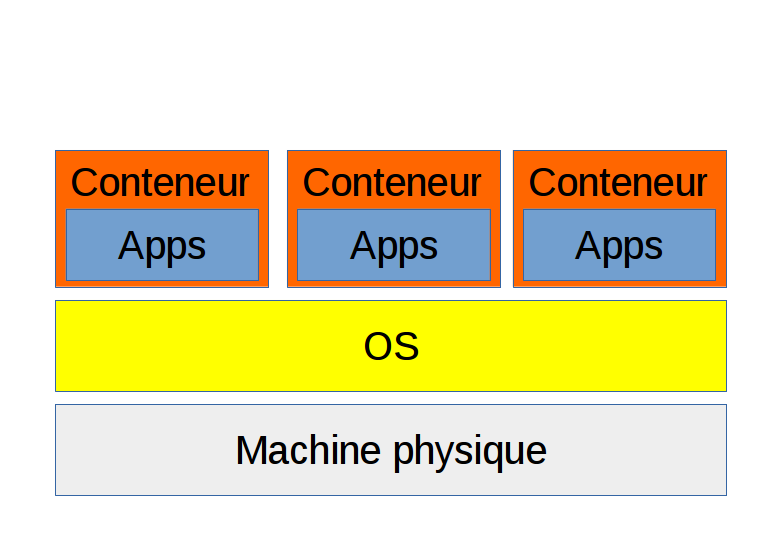
\includegraphics[width=\linewidth]{img/conteneur.png}
	\end{minipage}
	\hfill
	\begin{minipage}[b]{.49\textwidth}
		\begin{overprint}
			\only<2-7>{
				\begin{block}{Avantages}
					\begin{itemize}
						\item<2-> Portabilité des conteneurs (+ ou -)
						\item<3-> Isolations des applications (+ ou -)
						\item<4-> Mutualisations des ressources
						\item<5-> Ressources à la demande
						\item<6-> Démarrage quasiment aussi rapide qu'une application native	
						\item<7-> Contrairement aux VMs, pas d'overhead (économisation des ressources matérielles)	
					\end{itemize}
				\end{block}
			}
			\only<8-9>{
				\begin{alertblock}{Inconvénients}
					\begin{itemize}
						\item<8-> Ne permet d'exécuter que des applications compatibles avec le système hôte
						\item<9-> Peut-être sans état, volatile (dépend des technologies employées) $\Rightarrow$ pas de snapshot RAM incluse, pas de persistance des données nativement 
					\end{itemize}
				\end{alertblock}
			}
			\only<10-13>{
				\begin{alertblock}{Inconvénients (suite)}
					\begin{itemize}
						\item<10-> Certaines de ces technologies sont encore jeunes (docker, singularity)
						\item<11-> Courbe d'apprentissage un peu plus élevée que pour des VM
						\item<12-> Évolution très (trop ?) rapide
						\item<13-> Va-t-on vraiment vers un changement de paradigme ?
					\end{itemize}
				\end{alertblock}
				
			}
		\end{overprint}
	\end{minipage}
\end{frame}




\begin{frame}{Divers}
	On peut imbriquer plusieurs VM ou plusieurs conteneurs les uns dans les autres (en anglais nested virtualisation/containers)
\end{frame}

\begin{frame}
	\begin{exampleblock}{Chroot: le prémice de la conteneurisation}
		\only<1>{
			\begin{itemize}
			 	\item Réalisez un chroot pour un utilisateur d'uid 2000 sur un répertoire nommé new\_root. Vous aurez besoin de:
			 	\begin{itemize}
			 		\item chroot (et de man chroot)
			 		\item cp
			 		\item ldd
			 		\item mkdir
			 	\end{itemize}
			\end{itemize}					
		}
		\only<2>{
		\begin{shell}{}
			\prompt mkdir new\_root \\
 			\prompt cp -r /bin/ new\_root/ \\
			\prompt sudo chroot new\_root /bin/bash \\
			\prompt \# Zut alors\!
		\end{shell}
		}
		\only<3>{
		\begin{shell}{}
			\prompt ldd /bin/bash \\
			\prompt cp -r /lib new\_root/ \\
			\prompt cp -r /lib64 new\_root/ \\
			\prompt sudo chroot new\_root /bin/bash \\
			bash-4.3\# pwd \\
			/ \\
			bash-4.3\# echo \$UID \\
			0 \\
			bash-4.3\# exit \\
			\prompt
		\end{shell}
		}
		\only<4>{
		\begin{shell}{}
			\prompt sudo chroot --userspec 2000:2000 new\_root /bin/bash \\
			bash-4.3\# echo \$UID \\
			2000 \\
			bash-4.3\# ls -l / \# A vous de voir \\ 
			bash-4.3\# rm -r --no-preserve-root / \# A votre avis ? Et lorsque on ne met pas l'option userspec ?  \\
			bash-4.3\# exit \\
			\prompt
		\end{shell}
		}
	\end{exampleblock}
\end{frame}

\subsection{Des technologies de conteneurisations différentes pour des objectifs différents}
\begin{frame}{Les conteneurs applicatifs}
	\begin{block}{}
		Il s'agit des conteneurs qui ont pour objectif de n'exécuter qu'une application, qu'un service, voire même qu'un seul processus. Les deux principaux concurrents sont:
		\begin{itemize}
			\item Docker (Docker Inc.)
			\item Rocket (CoreOS Inc.)
		\end{itemize}
		Ce sont des technologies très prisées par le monde du DevOps (relation entre les développeurs et les administrateurs systèmes/réseaux).

		L'utilisation de ces technologies met en avant l'utilisation des architectures de micro-services (1 conteneur = 1 micro-service, multi-conteneurisation du service). Il s'agit de conteneur sans état (stateless), il n'y a pas de persistance de données par défaut, car ces conteneurs sont volatiles.
	\end{block}
\end{frame}

\begin{frame}{Les conteneurs pour l'administration système}
	\begin{block}{}
		Ce sont des conteneurs qui ont pour objectif de remplacer les VM. Ils diffèrent des conteneurs applicatifs dans le sens ou ils peuvent fournir un \textbf{ensemble} de (micro) services. Ce sont des conteneurs avec état (statefull): ils offrent une persistance des données et ils ont pour vocation d'être manipulés comme des VMs (snapshot, backup, migration à chaud). Les principaux concurrents sont:
		\begin{itemize}
			\item LXC (via LXD, Canonical)
			\item LXC (via Proxmox pct, Proxmox)
			\item OpenVZ
		\end{itemize}
		Les conteneurs LXC sont capables d'héberger des conteneurs Docker (sous conditions: voir \url{https://stgraber.org/2016/04/13/lxd-2-0-docker-in-lxd-712/}).
	\end{block}
\end{frame}

\begin{frame}{Les conteneurs pour le calcul haute performance}
	\begin{block}{}
		L'idée est de se servir du mécanisme des conteneurs pour offrir des environnements isolés mais performants dans le cadre du calcul haute performance. Singularity permet l'utilisation de conteneur à destination du HPC (utilisation sur des clusters de calculs). Les conteneurs singularity sont en mesure d’exécuter des conteneurs docker. Ils sont également plus sécurisés nativement et permettent l'utilisation native de certains protocoles (infiniband, openMPI, ...)
	\end{block}
\end{frame}


\section{Bases}
	\subsection{Introduction}
	\begin{frame}
		\begin{exampleblock}{La puissance de docker ?}
			Démonstration wordpress PWD
		\end{exampleblock}
	\end{frame}
	
	\begin{frame}{Contexte d’utilisation de docker}
	\begin{block}{}
	\begin{itemize}
	\item Dans le cadre du cours, notre utilisation de Docker se fera uniquement sur un noyau Linux. En effet, il existe une possibilité d'utiliser docker nativement sur Windows server 2016 et pour conteneuriser des applications windows.
	\pause
	\item On peut utiliser docker nativement sur un OS GNU / Linux. 
	\pause	
	\item On peut utiliser docker dans une machine virtuelle avec un os GNU/linux.
	\pause	
	\item On peut utiliser docker via une virtualisation Virtual Box minimale de l'os "boot2docker"via l'outil "docker toolbox" sur windows et macOS.
	\pause
	\item On peut avoir un environnement "bac à sable" docker en ligne avec l'excellent site "play with docker" (nécessite un compte docker)
	\end{itemize}
	
	\end{block}
	\end{frame}
		\begin{frame}
			\begin{block}{Historique}
				\begin{itemize}
					\item Solomon Hykes débute le projet Docker en interne pour DotCloud en France.
					\item Docker a été distribué en tant que projet open source à partir de mars 2013
					\item À partir de la version 0.9, Docker abandonne l'utilisation de LXC et développe sa propre librairie de conteneurs : libcontainer
					\item Docker est principalement développé par la société Docker Inc
					\item En 3 ans, 10 000 forks et 1400 contributeurs sur github pour le projet Docker
				\end{itemize}
			\end{block}
		\end{frame}
		\begin{frame}{Carte d'identité}
		\center
			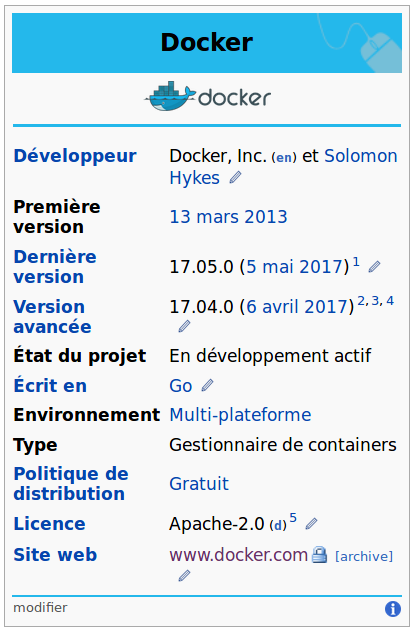
\includegraphics[height=5cm]{img/carte_identite.png}
		\end{frame}
		\begin{frame}{N.B: Versions de docker}
			\begin{alertblock}{}
				Il y a eu 2 grands changements majeurs dans l'historique de développements de docker:
				\begin{itemize}
					\item docker 0.9 $\Rightarrow$ fork de LXC pour création de libcontainer
					\item docker 1.10 $\Rightarrow$ Changement de gestion des images (4 février 2016)
				\end{itemize}
				\pause
				Ce cours a été fait sur la base de la version 17.03.1-ce. Les explications données ici peuvent être \textbf{incompatibles} avec les versions antérieures à docker 1.10. Si vous êtes amenés à consulter des forums sur internet, pensez à regarder la date du post et/ou la version de docker utilisée.
				\pause
				Plus d'informations sur ces changements majeurs:
				\begin{itemize}
					\item \url{https://blog.docker.com/2016/02/docker-1-10/}
					\item \url{http://windsock.io/explaining-docker-image-ids/}
				\end{itemize}
			\end{alertblock}
		\end{frame}
		\begin{frame}{}
			\only<1>{
				\begin{block}{Installation}
				\begin{itemize}
					\item Ubuntu 16.04 (VM ou natif)
					\item Dernière version stable de docker en CE (Community Edition)
					\item \url{https://docs.docker.com/engine/installation/linux/ubuntu/\#uninstall-old-versions}
					\item \url{https://docs.docker.com/engine/installation/linux/ubuntu/\#install-using-the-repository}
				\end{itemize}
				\end{block}
			}
			\only<2-3>{
				\begin{alertblock}{Pour ne pas avoir à écrire \textit{sudo} à chaque commande docker}
					\begin{shell}{}
						\prompt sudo usermod -aG docker \$USER \\
						\prompt \# Déconnexion, reconnexion \\
						\prompt systemctl enable docker \# Activation au démarrage de l'hôte
					\end{shell}
					\begin{itemize}
						\item<3> Considérez que vous êtes root à chaque fois que votre commande est préfixée par docker 
					\end{itemize}
				\end{alertblock}
			}
		\end{frame}
	\subsection{Définitions et prérequis}
		\begin{frame}{Définitions formelles}
		\vspace{-0.3cm}
			\begin{block}{Les images et les couches : bases des conteneurs docker}
				\begin{itemize}
					\item Une image désigne une collection \textbf{ordonnée} (par empilement) de \textbf{modifications} d'un système de fichiers racine.
					\pause
					\item On conserve chacune de ces modifications du FS dans \textbf{une couche ou un layer} identifiable par le hash sha256 de son contenu. $\Rightarrow$ Une image désigne donc une collection \textbf{ordonnée} de couche.
					\pause					
					\item A chaque couche \textbf{intermédiaire} est associé une image \textbf{intermédiaire}.
					\pause
					\item Les couches sont créées grâce à l'exécution de conteneurs qui sont transformés en image. (Pas de panique, on va faire un schéma)
					\pause
					\item Il peut y avoir des couches vides (empty layer).
					\pause
					\item Les couches désignées par une image sont nécessairement en lecture seule.
					\pause
					\item Une image est \textbf{unique}. Elle est identifiée par une fonction de hachage sha256 de son descriptif. Elle \textbf{n'a pas d'état} (i.e.: on n'exécute pas une image) et elle est \textbf{immuable}.
					\end{itemize}	
			\end{block}
		\end{frame}

		\begin{frame}{}
			\begin{block}{Un conteneur: l’instanciation d'une image}
				\begin{itemize}
				\item Le système de fichiers racine du conteneur \textbf{est} le système de fichiers racine de l'image sous-jacente, \textbf{mais} celui-ci est en lecture seule.
				\pause
				\item On a \textbf{l'illusion} de modifier le  système de fichiers racine dans le conteneur, car les changements sont effectuées dans \textbf{une nouvelle couche en lecture/écriture}. (technologie de Copy On Write (COW))
				\pause
				\item La suppression du conteneur entraîne \textbf{systématiquement la suppression de cette nouvelle couche en lecture/écriture}. 
				\pause
				\item On peut pérenniser les modifications effectuées dans le FS d'un conteneur en créant une \textbf{nouvelle} image qui va ajouter aux couches en lecture seule la nouvelle couche ainsi créée. La nouvelle couche qui était en lecture/écriture passe ainsi en lecture seule. 
				\pause
				\item Cette pérennisation se fait via la commande \textit{docker commit} 
				\end{itemize}
			\end{block}
		\end{frame}

		\begin{frame}
		\begin{alertblock}{Ce qu'il faut bien comprendre}
			\begin{itemize}
				\item Image $\neq$ Couche $\neq$ Conteneur
				\pause
				\item Une couche contient \textbf{uniquement} les \textbf{différences} d'un système de fichiers.
				\pause
				\item Un \textbf{ensemble} de couche peut former un système de fichiers racine.
				\pause
				\item Les couches ne savent rien des images qui les exploitent.
				\pause
				\item Les couches peuvent être utilisées par \textbf{plusieurs} images.
				\pause
				\item Une image peut faire référence à \textbf{plus d'1} couche.
				\pause
				\item Une image est quelque chose que vous pouvez instancier. Le \textbf{résultat} de cette instanciation est un conteneur.
				\pause
				\item Lorsque un conteneur démarre, certaines informations de l'image ayant permis son instanciation permettent de construire son système de fichiers racine.
			\end{itemize}						
		\end{alertblock}
		\normalsize
		\end{frame}		
	
		\begin{frame}{Représentation graphique}
		\vspace{-0.19cm}
			\only<1>{\includegraphics[width=\linewidth]{img/image_vs_conteneur_01.png}}
			\only<2>{\includegraphics[width=\linewidth]{img/image_vs_conteneur_02.png}}
			\only<3>{\includegraphics[width=\linewidth]{img/image_vs_conteneur_03.png}}
			\only<4>{\includegraphics[width=\linewidth]{img/image_vs_conteneur_04.png}}
			\only<5>{\includegraphics[width=\linewidth]{img/image_vs_conteneur_05.png}}
			\only<6>{\includegraphics[width=\linewidth]{img/image_vs_conteneur_06.png}}
			\only<7>{\includegraphics[width=\linewidth]{img/image_vs_conteneur_07.png}}
			\only<8>{\includegraphics[width=\linewidth]{img/image_vs_conteneur_08.png}}
			\only<9>{\includegraphics[width=\linewidth]{img/image_vs_conteneur_09.png}}
			\only<10>{\includegraphics[width=\linewidth]{img/image_vs_conteneur_10.png}}
			\only<11>{\includegraphics[width=\linewidth]{img/image_vs_conteneur_11.png}}
			\only<12>{\includegraphics[width=\linewidth]{img/image_vs_conteneur_12.png}}
			\only<13>{\includegraphics[width=\linewidth]{img/image_vs_conteneur_13.png}}
			\only<14>{\includegraphics[width=\linewidth]{img/image_vs_conteneur_14.png}}
		\end{frame}
		
		\begin{frame}
		\begin{alertblock}{Images particulières}
			\begin{itemize}
				\item Une "top level image" n'est pas une image intermédiaire
				\pause
				\item Une image taguée "none" est une image intermédiaire, sinon c'est une top level image pendante (dangling)
				\pause
				\item Une image taguée "missing" est une image manquante mais dont on a obtenu le layer associé (via \textit{docker pull})
				\pause
			\end{itemize}
			\end{alertblock}
			\begin{alertblock}{Avant la version 1.10}
			\begin{itemize}
				\item Chaque image était identifiée par un nombre aléatoire
				\pause 
				\item Chaque image était associée à \textbf{1 seule} couche.
				\pause
				\item $\Rightarrow$ Chaque couche était repérée par le même identifiant que l'image
				\pause
				\item $\Rightarrow$ Problèmes de sécurité à cause du nombre aléatoire
				\pause
				\item Pour plus d'informations: \url{http://windsock.io/explaining-docker-image-ids/}
			\end{itemize}
				
			\end{alertblock}
		\end{frame}
		
		\begin{frame}{Quelques commandes de bases}
			\begin{block}{Gestion des images}
				\begin{itemize}
					\item \textit{docker pull}: télécharger une image présente sur un registre (docker hub par défaut)
					\item \textit{docker push}: pousser (upload) une image sur un registre
					\item \textit{docker search}: chercher une image sur un registre
					\item \textit{docker images}: liste les images présentes localement
					\item \textit{docker history}: affiche l'historique de création d'une image
					\item \textit{docker rmi}: supprimer une image
					\item \textit{docker commit}: construire une image à partir d'un conteneur
					\item \textit{docker build}: construire une image à partir d'un dockerfile
				\end{itemize}
			\end{block}
		\end{frame}
		\begin{frame}{Quelques commandes de bases}
			\begin{block}{Gestion des conteneurs}
				\begin{itemize}
					\item \textit{docker run}: démarrer un conteneur
					\item \textit{docker stop/start/restart/pause/unpause}: arrête/démarre/redémarre/pause/reprise d'un conteneur
					\item \textit{docker logs}: obtenir les journaux système d'un conteneur
					\item \textit{docker kill}: tuer un conteneur
					\item \textit{docker rm}: supprimer un conteneur
					\item \textit{docker ps}: liste les conteneurs actifs
				\end{itemize}
			\end{block}
		\end{frame}

		\begin{frame}{Quelques commandes de bases}
			\begin{alertblock}{Plusieurs commandes pour le même résultat}
				\begin{itemize}
					\item Les commandes vues précédemment sont les commandes historiques de docker
					\item Avec le temps, docker a regroupé ses commandes en fonction des "objets" concernés
					\item Par exemple, toutes les commandes concernant: 
					\begin{itemize}
						\item les conteneurs sont regroupées dans \textit{docker container cmd}
						\item les images sont regroupées dans \textit{docker image cmd}
						\item et ainsi de suite pour: config, container, image, network, node, plugin, secret, service, stack, swarm, system et volume
					\end{itemize}
					\item Mais \textit{docker container ls -aq} \textbf{est identique à} \textit{docker ps -aq}
					\item Etc, etc
				\end{itemize}
			\end{alertblock}
		\end{frame}
		
		\begin{frame}{Quelques commandes de bases}
			\begin{block}{Gestion de docker}
				\begin{itemize}
					\item \textit{docker info}: affiche des informations relatives à l'écosystème docker sur la machine
					\item \textit{docker inspect}: affiche des informations de bas niveau sur des objets docker (images, conteneurs, réseaux, ...)
					\item \textit{docker version}: affiche la version de docker
				\end{itemize}
			\end{block}
		\end{frame}
		\begin{frame}{"Philosophie" de docker: Bonnes pratiques recommandées}
			\begin{block}{}
				\begin{itemize}
					\item Un conteneur doit être éphémère (séparation et point de montage des données dans le conteneur)
					\pause
					\item Un conteneur = 1 (micro) service (= 1 processus pour les puristes)
					\pause
					\item On ne devrait pas être root dans un conteneur (sshd, crond, firewall, ... $\Rightarrow$ Hôte)
					\pause
					\item Si jamais on doit être root, utilisation d'un setuid, gosu ou su-exec
					\pause
					\item Minimiser la taille des images (pas de superflu)
					\pause
					\item Minimiser le nombre de couches dans une image (Dockerfile $\Rightarrow$ multi-ligne argument, pipe)
					\pause
					\item Maximiser le partage des couches
					\pause
					\item Les couches les plus volumineuses au plus près de la racine (utilisation du cache de \textit{docker build})
				\end{itemize}
			\end{block}
		\end{frame}
		
		\begin{frame}{"Philosophie\textbf{s}" de docker ?}
		\begin{block}{}
				\begin{itemize}
					\item Adapter les bonnes pratiques en fonction de ses besoins et de ses usages
					\pause
					\item Pour plus d'un processus par conteneur, voir du côté de supervisor
					\pause
					\item Utilisez-vous la bonne technologie de conteneurisation ?
				\end{itemize}
			\end{block}
		\end{frame}



	\subsection{Premiers pas}
		\begin{frame}{Notre premier conteneur}
			\begin{exampleblock}{Hello world !}
				\begin{shell}{}
				\small
				\only<1>{\begin{text}
						\prompt docker run hello-world \\
						Unable to find image 'hello-world:latest' locally\\
						latest: Pulling from library/hello-world\\
						78445dd45222: Downloading [===============\textgreater \ \ \ \ \ \ \ \ \ \ \ \ \ \ ] \\
					\end{text}
				}
				\only<2>{\begin{text}
						\prompt docker run hello-world \\
						Unable to find image 'hello-world:latest' locally\\
						latest: Pulling from library/hello-world\\
						78445dd45222: Extracting \ \ \ [=========\textgreater \ \ \ \ \ \ \ \ \ \ \ \ \ \ \ \ \ \ \ \ \ \ \ \ \ \ \ ] \\
					\end{text}
				}
				\only<3>{\begin{text}
						\prompt docker run hello-world \\
						Unable to find image 'hello-world:latest' locally\\
						latest: Pulling from library/hello-world\\
						78445dd45222: Pull complete \\
						Digest: sha256:c5515758d4c5e1e838e9cd307f6c6a0d620b5e07e6f927b07d05f6d12a1ac8d7\\
						Status: Downloaded newer image for hello-world:latest\\
						...
					\end{text}
				}
				\tiny
				% A PROPOS DU CONTENEUR 4-8
				\only<4>{\begin{shellContainer}{} \verbatiminput{output/hello-world.txt} \end{shellContainer}}
				\only<5-8> {
					\begin{text} \prompt docker ps\\ \end{text}
					\begin{text} \prompt docker ps -a \end{text}
					\verbatiminput{output/hello_ps.txt}
					%\end{verbatim}
					\begin{text} \prompt docker ps -aq\\
					ccdd8f78bf58\\
					\end{text}
					\begin{text} \prompt docker inspect --format='\{\{.ID\}\}' furious\_pare\\
					ccdd8f78bf58e744968462d979bde759155dcd6892cad94bea2bf64fe3fa0012\\
					\end{text}
				}
				% A PROPOS DE L'IMAGE 9-12
				\only<9-12> {
					\begin{text} \prompt docker images \end{text}
					\verbatiminput{output/hello_image.txt}
					\begin{text} \prompt docker images -aq \\ 48b5124b2768\\ \end{text}
					\begin{text} \prompt docker inspect --format='\{\{.ID\}\}' hello-world \\
					sha256:48b5124b2768d2b917edcb640435044a97967015485e812545546cbed5cf0233	\\
					\end{text}
					\begin{text} \prompt docker inspect --format='\{\{.RootFS.\textit{layers}\}\}' hello-world
					$[$sha256:98c944e98de8d35097100ff70a31083ec57704be0991a92c51700465e4544d08$]$ \\
					\end{text}
				}
				% A PROPOS DE LA SUPPRESSION ET DES IDENTIFIANTS 12-18
				\only<13> {
					\begin{text} \prompt docker rm furious\_pare \# docker rm ccdd8 (debut CONTAINER ID)\\
				        furious\_pare \\ \end{text}
				}
				\only<14-18> {
					\begin{text} \prompt docker rmi hello-world \# docker rmi 48b (debut IMAGE ID)\\
				        Untagged: hello-world:latest\\
					Untagged: hello-world@sha256:c5515758d4c5e1e838e9cd307f6c6a0d620b5e07e6f927b07d05f6d12a1ac8d7\\
					Deleted: sha256:48b5124b2768d2b917edcb640435044a97967015485e812545546cbed5cf0233\\
					Deleted: sha256:98c944e98de8d35097100ff70a31083ec57704be0991a92c51700465e4544d08\\
			       		\end{text}
				}
			       \end{shell}
				\vspace{-0.3cm}

				\only<5-8> {
					\begin{enumerate}
						\item<5-8> Aucun conteneur actif
						\item<6-8> 1 conteneur inactif (-a = all), si nom non spécifié, attribution d'un nom aléatoire
						\item<7-8> (-q = quiet)
						\item<8>  CONTAINER ID affecté aléatoirement
					\end{enumerate}
				}
				\only<9-12>{
					\begin{enumerate}
						\item<9-12>  Liste les images de plus haut niveau (top level image)
						\item<10-12>  Liste de façon silencieuse (-q) toutes les images (intermédiaires également) 
						\item<11-12>  IMAGE ID affecté par fonction de hachage 
						\item<12> Fonction de hachage du layer décompressé (N.B.: présence des $[]$)
					\end{enumerate}
				}

				\only<13>{
					\begin{itemize}
						\item Suppression du conteneur par son nom ou son identifiant
					\end{itemize}
				}
		
				\only<14-18>{
					\begin{itemize}
						\item<14-18> latest considéré comme tag par défaut (untagged by user)
						\item<15-18> hello-world@sha256:c55...  considéré comme tag par défaut (untagged by user)(Hash Image Compressed)
						\item<16-18> Deleted: sha256:48b... $\Rightarrow$ Suppression de l'image
						\item<17-18> Deleted: sha256:98c... $\Rightarrow$ Suppression des couches de l'image (1 seule en l’occurrence) car couches non partagées par d'autres images.
						\item<18> A quoi correspond 78445dd45222 lors du pull ? $\Rightarrow$ Hash Layer Compressed
					\end{itemize}
				}
			\end{exampleblock}
		\end{frame}

\begin{frame}{Quelques cas faciles}
	\vspace{-0.3cm}
	\begin{exampleblock}{Quelques conteneurs à exécuter}
	Prenez le temps de lancer quelques conteneurs simplement, par exemple:
		\begin{enumerate}
			\item Exécutez "/bin/bash" dans un conteneur interactif ubuntu
			\item Exécutez "/bin/ls" dans un conteneur non interactif ubuntu
			\item Exécutez "/bin/ps -eflH" dans un conteneur non interactif ubuntu
			\item Exécutez "/bin/bash" dans un conteneur interactif nommé "mon\_conteneur\_c0" ubuntu
			\item Détachez-vous du conteneur "mon\_conteneur\_c0" avec Crtl+p Ctrl+q
			\item Rattachez-vous au conteneur "mon\_conteneur\_c0"
			\item Sortez du conteneur "mon\_conteneur\_c0"
			\item Listez les conteneurs actifs, listez tous les conteneurs
			\item Supprimez tous les conteneurs inactifs en 1 commande (\textit{docker container help})
		\end{enumerate}
	\end{exampleblock}
\end{frame}

\begin{frame}{Quelques cas faciles: commentaires}
	\vspace{-0.3cm}
	\begin{exampleblock}{Quelques conteneurs à exécuter}
	Prenez le temps de lancer quelques conteneurs simplement, par exemple:
		\begin{enumerate}
			\item \textit{docker run -it ubuntu /bin/bash}
			\item \textit{docker run ubuntu /bin/ls}
			\item \textit{docker run ubuntu /bin/ps -eflH}
			\item \textit{docker run -it --name mon\_conteneur\_c0 ubuntu}
			\item Ctrl+p Ctrl+q
			\item \textit{docker container attach mon\_conteneur}
			\item \textit{exit}
			\item \textit{docker container ls; docker container ls -a}
			\item \textit{docker container prune}
		\end{enumerate}
	\end{exampleblock}
\end{frame}

\begin{frame}{Quelques cas pénibles}
	\vspace{-0.3cm}
	\begin{exampleblock}{Quelques conteneurs à exécuter}
	Vous utiliserez les commandes \textit{docker run} et \textit{docker container}.\\
	\textit{docker cmd help} pour l'aide sur la commande \textit{cmd}
		\begin{enumerate}
			\item Essayez d'exécuter "/bin/bash" dans un conteneur interactif alpine
			\item Exécutez "echo hello world !" dans un conteneur non interactif centos "c1" 
			\item Essayez de démarrer 1 fois le conteneur "c1". Faites \textit{docker logs c1}
			\item Exécutez "\textit{/bin/bash}" dans un conteneur non interactif centos "c2"
			\item Essayez de démarrer 1 fois le conteneur "c2". Faites \textit{docker logs c2}
			\item Exécutez "\textit{/bin/bash}" dans un conteneur interactif centos "c3" et \textit{exit} de c3
			\item Démarrez, connectez vous avec un nouveau bash et détachez vous du conteneur "c3"
			\item Listez les processus du conteneur "c3" depuis l'hôte \textbf{et} depuis le conteneur (ps)
		\end{enumerate}
	\end{exampleblock}
\end{frame}

\begin{frame}{Quelques cas pénibles: commentaires}
	\vspace{-0.3cm}
	\begin{exampleblock}{}
	Vous utiliserez les commandes \textit{docker run} et \textit{docker container}.\\
	\textit{docker cmd help} pour l'aide sur la commande \textit{cmd}
		\begin{enumerate}
			\item /bin/bash n'est pas présent par défaut dans alpine (Idée sous-jacente: 
			\begin{itemize}
				\item Minimiser la taille des images, on n'installe que ce dont a besoin
				\item La distribution Alpine fait 5 Mo !
			\end{itemize} 
			\item \textit{docker run centos echo hello world !}
			\item c1 est en mode non interactif et "echo" est sans boucle d'événement, mais "\textit{hello}" effectué réellement 2 fois.
			\item c2 est en mode non interactif et il n'y a pas de pseudo-terminal alloué
			\item La commande "\textit{/bin/bash}"  est effectué réellement 2 fois
			\item \textit{docker run -it --name c3 centos /bin/bash; exit;} 
			\item \textit{docker start c3; docker exec -it c3 /bin/bash; Ctrl+p Ctrl+q} 
			\item \textit{docker container top c3; docker exec c3 ps;} PID host, PID guest
		\end{enumerate}
	\end{exampleblock}
\end{frame}
	\subsection{Volatilité, persistance et sécurité des données}
		\begin{frame}{Volatilité, persistance et sécurité des données}
			\begin{exampleblock}{Something more ambitious}
				\only<1>
				{
					\begin{shell}{}
						\prompt docker run -it ubuntu /bin/bash \\
						Unable to find image 'ubuntu:latest' locally \\
						latest: Pulling from library/ubuntu \\
						bd97b43c27e3: Pull complete  \\
						6960dc1aba18: Pull complete  \\
						2b61829b0db5: Pull complete  \\
						1f88dc826b14: Pull complete  \\
						73b3859b1e43: Pull complete  \\
						Digest: sha256:ea1d854d38be82f54d39efe2c67000bed1b03348bcc2f3dc094f260855dff368 \\
						Status: Downloaded newer image for ubuntu:latest \\
					\end{shell}
				}
			
				\only<2>
				{
					\begin{shell}{}
						\begin{shellContainer}{}
							root@dfdf734253a9:/\# ls\\
							bin  boot  dev  etc  home  lib  lib64  media  mnt  opt  proc  root  run  sbin  srv  sys  tmp  usr  var\\
							root@dfdf734253a9:/\# rm -rf / \# Aucune incidence sur  l'hôte car pas de montage de volume\\
							rm: it is dangerous to operate recursively on '/' \\
							rm: use --no-preserve-root to override this failsafe \\
						\end{shellContainer}
					\end{shell}
				}
				\only<3>
				{
					\begin{shell}{}
						\begin{shellContainer}{}
							root@dfdf734253a9:/\# rm -rf --no-preserve-root / \\
							... \\
							rm: cannot remove '/proc/fs/aufs/plink\_maint': Read-only file system \\
							... \\
							root@dfdf734253a9:/\# ls \\
							bash: /bin/ls: No such file or directory \\
							root@dfdf734253a9:/\# exit \\
						\end{shellContainer}
						\prompt 
					\end{shell}
				}
				\only<4>
				{
					\begin{shell}{}
						\prompt docker ps -a \\
						\tiny
						\verbatiminput{output/ps_secure_example.txt}
						\normalsize
						\prompt docker rm dfd \\
						dfd\\
						\prompt
					\end{shell}
				}
				\only<5>
				{
					\begin{shell}{}
						\prompt docker run -it ubuntu /bin/bash\\
						\vspace{0,2cm}
						\begin{shellContainer}{}
							root@\textcolor{red}{63f0abcc808a}:/\# \textcolor{red}{\#Ceci est un nouveau conteneur\\}
							root@63f0abcc808a:/\# ls\\
							bin  boot  dev  etc  home  lib  lib64  media  mnt  opt  proc  root  run  sbin  srv  sys  tmp  usr  var\\
							root@63f0abcc808a:/\# exit
						\end{shellContainer}
						\prompt
					\end{shell}
				}
				\only<6>
				{
					\begin{shell}{}
						\prompt docker ps -a \\
						\tiny
						\verbatiminput{output/ps_secure_example2.txt}
						\normalsize
						\prompt docker rm suspicious\_goldstine \\
						suspicious\_goldstine\\
						\prompt
					\end{shell}
				}
				\only<7>
				{
					\begin{shell}{}
						\prompt docker run -it -v /:/danger\_racine\_hote --hostname myhostname --name myname ubuntu /bin/bash
						\vspace{0,2cm}
						\begin{shellContainer}{}
							root@myhostname:/\# ls\\
							bin  boot  dev  etc  home  lib  lib64  media  mnt  opt  proc  danger\_racine\_hote  root  run  sbin  srv  sys  tmp  usr  var \\
							root@myhostname:/\# ls /danger\_racine\_hote\\
							bin  boot  cdrom  dev  etc  home  initrd.img  lib  lib64  lost+found  media  mnt  opt  proc  root  run  sbin  srv  sys  tmp  usr  var  vmlinuz \\
							root@myhostname:/\# \# \textcolor{red}{Ne pas faire rm -rf /danger\_racine\_hote :-0}
						\end{shellContainer}
					\end{shell}
				}
				\only<8>
				{
					\begin{shell}{}
						\prompt docker ps -a \\
						\tiny
						\verbatiminput{output/ps_secure_example3.txt}
						\normalsize
						\prompt docker rm myname \\
						myname\\
						\prompt
					\end{shell}
				}
				\only<9>
				{
					\begin{shell}{}
						\prompt docker run -it \textcolor{red}{--rm} ubuntu /bin/bash\\
						\vspace{0.5cm}
						\begin{shellContainer}{}
						root@30481297b94c:/\# exit
						\end{shellContainer}
						\prompt docker ps -a\\
						\tiny
						\verbatiminput{output/ps_secure_example4.txt}
						\normalsize
						\prompt
					\end{shell}
				}
			\end{exampleblock}
	\end{frame}
	\normalsize
	\begin{frame}{Volatilité, persistance et sécurité des données}	
		\begin{block}{Résumé}
			\begin{itemize}
				\item Il peut être dangereux d'exécuter des conteneurs contenant des processus root
				\pause
				\item On peut monter des répertoires de l'hôte dans le conteneur afin d'assurer la persistance de certaines données
				\pause
				\item Cette technologie de persistance s’appelle data volume
				\pause
				\item Pour des montages sur des ressources partagées (NFS, ISCSI, FC): voir docker volume plugin
				\pause
				\item Il existe une technologie de persistance à travers des conteneurs: data volume container
			\end{itemize}
		\end{block}
	\end{frame}

	\subsection{Sécurité des conteneurs}
	\begin{frame}{Sécurité des conteneurs}
	\vspace{-0.3cm}
		\begin{alertblock}{Namespace: isolation de base}
			\begin{itemize}
				\item Les processus exécutés dans un conteneur ne peuvent ni voir ni affecter les processus exécutés dans un autre conteneur ou dans le système hôte.
				\pause
				\item Chaque conteneur possède son propre réseau. Si l'hôte est configuré en conséquence, les conteneurs peuvent interagir les uns avec les autres (et avec l'hôte) au travers de leurs interfaces de réseau respectives
				\pause
				\item Tous les conteneurs d'un hôte Docker sont connectés à des bridges (virtual switch).
				\pause
				\item Il est tout de même déconseillé d'utiliser des applications root (ssh, vpn, dhcp, ...). L'hôte étant supposé subvenir à ces besoins.
				\pause
				\item Si on souhaite modifier le comportement par défaut de l'isolation, cela implique une intervention et une connaissance des "capabilities" (c'est un prix à payer lorsque l'on partage le même noyau)
				\pause
				\item Plus d'info sur \url{https://docs.docker.com/engine/security/security/}
			\end{itemize}
		\end{alertblock}
	\end{frame}
	
	\begin{frame}{Sécurité des conteneurs}	
		\begin{alertblock}{Capabilities}
			\begin{itemize}
				\item Il peut être dangereux d'exécuter des conteneurs contenant des processus root
				\pause
				\item En cas d'escalade de privilège depuis le conteneur sur l'hôte: par défaut le root dans le conteneur n'a pas les mêmes droits que le potentiel root sur l'hôte.
				\pause
				\item En effet celui-ci ne dispose pas de toutes les capabilities.
				\pause
				\item Plus d'info sur \url{https://linux.die.net/man/7/capabilities}
			\end{itemize}
		\end{alertblock}
	\end{frame}
	
	\begin{frame}{Sécurité des conteneurs}	
		\begin{alertblock}{Capabilities par défaut}
				\begin{columns}
					\begin{column}{150px}
						\begin{itemize}
							\item CAP\_CHOWN
							\item CAP\_DAC\_OVERRIDE
							\item CAP\_FSETID
							\item CAP\_FOWNER
							\item CAP\_MKNOD
							\item CAP\_NET\_RAW
							\item CAP\_SETGID
						\end{itemize}
					\end{column}
					\begin{column}{150px}
						\begin{itemize}
							\item CAP\_SETUID
							\item CAP\_SETFCAP
							\item CAP\_SETPCAP
							\item CAP\_NET\_BIND\_SERVICE
							\item CAP\_SYS\_CHROOT
							\item CAP\_KILL
							\item CAP\_AUDIT\_WRITE
						\end{itemize}
					\end{column}
				\end{columns}
		\end{alertblock}
	\end{frame}
	
	\begin{frame}{Sécurité des conteneurs}	
		\begin{alertblock}{CGroups: limitations des ressources}
			\begin{itemize}
				\item Comptabilité et limitations des ressources par conteneur
				\pause
				\item Par défaut: part équitable de ressources (CPU, RAM, I/O) par conteneur
				\pause
				\item Empêche l'utilisation de toutes les ressources par un conteneur (démo fork bomb --cpuset-cpus 0)
				\pause
				\item D'une certaine manière, ils empêchent certaines attaques de type DOS
				\pause
				\item "Garantit" une disponibilité et une performance quasiment constante
			\end{itemize}
		\end{alertblock}
	\end{frame}	
	
	\begin{frame}{Démon docker}	
		\begin{alertblock}{Surface d'attaque}
			\begin{itemize}
				\item Le démon docker est exécuté en root !
				\pause
				\item Seul un administrateur devrait pouvoir contrôler ce démon. (quid wrapper)
				\pause
				\item Quelle confiance accordez vous à l'image docker que vous téléchargez ?
				\pause
				\item Il est recommandé de n'utiliser que docker sur un serveur (à part ssh, dhcp, etc, s'il y a d'autres applications, il faut les conteneuriser ou il faut les déplacer)
				\pause
				\item Il ne faut pas faire ses tests de conteneur sur une machine de prod !
			\end{itemize}
		\end{alertblock}
	\end{frame}	

	\subsection{Conteneurs graphiques}
		\begin{frame}{C'est possible}
			\begin{itemize}
			 	\item Il est tout à fait possible d'exécuter des conteneurs graphiques (skype dans un conteneur par exemple).
			 	\item En général, on fait un mapping de /tmp/.X11-unix et de ~/.Xauthority de l'hôte vers le conteneur avec Xorg.
			 	\item Certains utilisent vnc (beaucoup moins efficace, mais plus sécurisé ...).
			 	\item Quid de Wayland ?
			 	\item Nous n'aborderons pas plus cet aspect dans ce cours.
			\end{itemize}		
		\end{frame}

\section{Utilisation avancées}
	\subsection{Créations d'images: méthode naïve}
		\begin{frame}{La méthode naïve}
			\begin{alertblock}{3 cas d'usage}	
			\begin{itemize}
				\item Pour un usage pédagogique
				\item Lorsque l'on n'est pas en mesure de configurer un environnement autrement qu'en mode graphique :-( (éclipse par exemple)
				\item Pour déboguer une construction automatisée (\textit{docker build})
			\end{itemize}
			\end{alertblock}
		\end{frame}

		\begin{frame}{La méthode naïve}
			\begin{exampleblock}{Utilisation de docker commit}
				\only<1>
				{
					\begin{shell}{}
						\prompt docker run -it -h conteneur --name conteneur\_avant\_commit ubuntu /bin/bash\\
						\vspace{0,2cm}
						\begin{shellContainer}{}
							root@conteneur:/\# echo "hello world !" \textgreater /nouveau\_fichier\_dans\_le\_systeme\_de\_fichier\_racine.txt\\
							root@conteneur:/\# exit\\
							exit\\
						\end{shellContainer}
					\end{shell}
				}
				\only<2>
				{
					\begin{shell}{}
						\small
						\prompt docker images
						\verbatiminput{output/docker_images_first1.txt}
						\prompt docker commit conteneur\_avant\_commit image\_apres\_commit\_du\_conteneur\\
						sha256:ca0028fa88252c281db33655b17517f3484b82ae42057e26193a6b91045bf2b8\\
						\prompt docker images
						\footnotesize
						\verbatiminput{output/docker_images_first2.txt}
						\normalsize

					%	\vspace{0,2cm}
					%	\begin{shellContainer}{}
					%	\end{shellContainer}
					\end{shell}
				}
				\only<3>
				{
					\begin{shell}{}
						\prompt docker run --rm image\_apres\_commit\_du\_conteneur cat /nouveau\_fichier\_dans\_le\_systeme\_de\_fichier\_racine.txt\\

						\vspace{0,2cm}
						\begin{shellContainer}{}
							hello world !
						\end{shellContainer}
						\prompt
						\normalsize
					\end{shell}
				}
			\end{exampleblock}
		\end{frame}
		
		\begin{frame}{La méthode naïve}
			\begin{exampleblock}{A vous}
				\begin{itemize}
					\item Faire une image "mon\_image" à partir d'une ubuntu 16.04
					\item Cette nouvelle image contiendra le paquet inetutils-ping
					\item Tester la commande "\textit{docker run mon\_image ping localhost}"
				\end{itemize}	
			\end{exampleblock}
			\small
			\begin{alertblock}{Problème de résolution DNS dans certains sous-réseaux}
				Il se peut que votre réseau vous oblige à passer par un DNS précis. Ce DNS précis ne correspond pas forcément aux adresses présentes dans /etc/resolv.conf de l'hôte (surcharge effectuée par network manager). Dans ce cas, la résolution de nom ne se fera pas dans le conteneur (et vous ne pourrez pas installer de paquets), car la surcharge de network manager n'affectera pas le conteneur (qui lui s'en tiendra au fichier /etc/resolv.conf). De fait, il vous faut soit changer le contenu de /etc/resolv.conf, soit passer l'argument --dns IP\_DNS lors du lancement du conteneur. Il préférable, pour la suite, de privilégier l'ajout du serveur DNS dans le fichier /etc/resolv.conf de l'hôte. Pour obtenir IP\_DNS, vous pouvez utiliser l'utilitaire nmcli (network manager command line interface), en général: \textit{nmcli device show $|$ grep DNS}.
			\end{alertblock}
			\normalsize
		\end{frame}

\subsection{Créations d'images: Dockerfile}
		\begin{frame}{La méthode efficace: Dockerfile}
			\begin{block}{}
				\begin{itemize}
					\item Un Dockerfile est un document texte contenant toutes les commandes que vous exécuteriez normalement manuellement sur un OS (apt/yum, configurations de logiciels, créations d'utilisateurs, variables d'environnements, ...).
					\pause					
					\item Avec la commande \textit{docker build}, docker peut créer des images \textbf{automatiquement} en lisant les instructions d'un Dockerfile.
					\pause
					\item A \textbf{chaque} instructions du dockerfile, docker build génère une image  et un layer si nécessaire (car potentiellement vide), on parle d'image intermédiaire, sauf pour la dernière instruction, qui correspond à l'image finale (top level image).
					\pause
					\item Les images intermédiaires sont générées par un mécanisme de commit des conteneurs dans lesquels les instructions ont été exécutées.
					\pause
					\item On peut créer plusieurs images avec un seul Dockerfile (mais on ne devrait pas)
				\end{itemize}
			\end{block}
		\end{frame}

		\begin{frame}{La méthode efficace: Dockerfile}
			\begin{block}{}
				\begin{itemize}
					\item Il faut dédier un répertoire pour chaque création d'image par dockerfile. En effet, docker build fonctionne avec une notion de contexte qui s'applique récursivement à partir du chemin (path) du répertoire contenant le Dockerfile.
					\item \textcolor{red}{Il ne faut surtout pas créer un Dockerfile à la racine du système. En effet, le contexte envoyé au démon docker concernerait l'intégralité du système de fichiers !}
					\item À l'instar de git, vous pouvez utiliser un fichier .dockerignore.
					\item docker build ignorera tous les fichiers/répertoires indiqués dans .dockerignore (i.e. ils ne feront pas partie du contexte).
					\item Les commentaires dans un Dockerfile sont préfixés par \#.
				\end{itemize}
			\end{block}
		\end{frame}
		
		\begin{frame}{La méthode efficace: Dockerfile}
			\begin{block}{}
				\begin{itemize}
					\item Il est possible d'utiliser des variables interprétables par certaines instructions dans un Dockerfile.
					\item Ces variables sont des variables d'environnement (comme HOME, PATH, ...)
				\end{itemize}
			\end{block}
		\end{frame}

		\begin{frame}{La méthode efficace: Dockerfile}
		\vspace{-0.15cm}
			\begin{block}{Liste des instructions possibles}
				\begin{columns}
					\begin{column}{150px}
						\begin{itemize}
							\item FROM
							\item RUN
							\item CMD
							\item \textcolor{green}{LABEL}
							\item MAINTAINER (déprécié, utiliser LABEL)
							\item \textcolor{green}{EXPOSE}
							\item \textcolor{green}{ENV}
							\item \textcolor{green}{ADD}
							\item \textcolor{green}{COPY}
						\end{itemize}
					\end{column}
					\begin{column}{150px}
						\begin{itemize}
							\item ENTRYPOINT
							\item \textcolor{green}{VOLUME}
							\item \textcolor{green}{USER}
							\item \textcolor{green}{WORKDIR}
							\item ARG
							\item \textcolor{green}{ONBUILD}
							\item \textcolor{green}{STOPSIGNAL}
							\item HEALTHCHECK
							\item SHELL
						\end{itemize}
					\end{column}
				\end{columns}
				\vspace{0,2 cm}
				\centering
				\textcolor{green}{Capables d'interpréter les variables d'environnement}
			\end{block}
		\end{frame}
		\begin{frame}{La méthode efficace: Dockerfile}
		\vspace{-0.3cm}
			\begin{exampleblock}{Dockerfile d'un serveur ssh}
			%	\tiny
			%	\begin{columns}[t]
			%		\begin{column}{150px}
			%			\verbatiminput{src/dockerfile_sshd1}
			%		\end{column}
			%		\begin{column}{150px}
			%			\verbatiminput{src/dockerfile_sshd2}
			%		\end{column}
			%	\end{columns}
			%	\normalsize
			\centering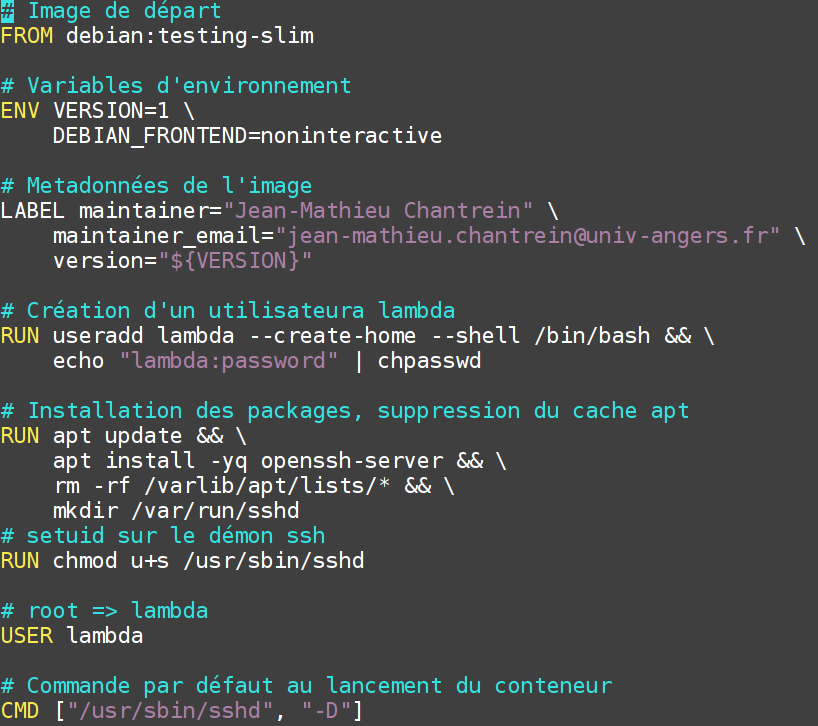
\includegraphics[width=6.8cm]{img/dockerfile_sshd.png}
			\end{exampleblock}
		\end{frame}

		\begin{frame}{La méthode efficace: Dockerfile}
			\begin{exampleblock}{Dockerfile serveur ssh: /home/jmc/sshd/Dockerfile}
				\tiny
				\only<1>
				{
					\begin{shell}{}
						\promptsshd docker build . -t sshd
						\verbatiminput{output/build_dockerfile_sshd1.txt}	 %\end{verbatim}	<-- Ne pas enlever, bug coloration syntaxique
					\end{shell}
				}
				\only<2>
				{
					\begin{shell}{}
						\verbatiminput{output/build_dockerfile_sshd2.txt} %\end{verbatim}	<-- Ne pas enlever, bug coloration syntaxique
						\promptsshd
					\end{shell}
				}
				\normalsize
			\end{exampleblock}
		\end{frame}
	
%\end{verbatim}	<-- Ne pas enlever, bug coloration syntaxique							
		
		\begin{frame}{La méthode efficace: Dockerfile}
			\begin{exampleblock}{Dockerfile serveur ssh: explication graphique}
				\only<1>{\includegraphics[width=\linewidth]{img/build_sshd_01.png}}
				\only<2>{\includegraphics[width=\linewidth]{img/build_sshd_02.png}}
				\only<3>{\includegraphics[width=\linewidth]{img/build_sshd_03.png}}
				\only<4>{\includegraphics[width=\linewidth]{img/build_sshd_04.png}}
				\only<5>{\includegraphics[width=\linewidth]{img/build_sshd_05.png}}
				\only<6>{\includegraphics[width=\linewidth]{img/build_sshd_06.png}}
				\only<7>{\includegraphics[width=\linewidth]{img/build_sshd_07.png}}
				\only<8>{\includegraphics[width=\linewidth]{img/build_sshd_08.png}}
				\only<9>{\includegraphics[width=\linewidth]{img/build_sshd_09.png}}
				\only<10>{\includegraphics[width=\linewidth]{img/build_sshd_10.png}}
				\only<11>{\includegraphics[width=\linewidth]{img/build_sshd_11.png}}
				\only<12>{\includegraphics[width=\linewidth]{img/build_sshd_12.png}}
				\only<13>{\includegraphics[width=\linewidth]{img/build_sshd_13.png}}
				\only<14>{\includegraphics[width=\linewidth]{img/build_sshd_14.png}}
				\only<15>{\includegraphics[width=\linewidth]{img/build_sshd_15.png}}
			\end{exampleblock}
		\end{frame}
		
		\begin{frame}{La méthode efficace: Dockerfile}
		\vspace{-0.3cm}
			\begin{exampleblock}{Dockerfile d'un serveur ssh: notions de contexte et de cache}
				\centering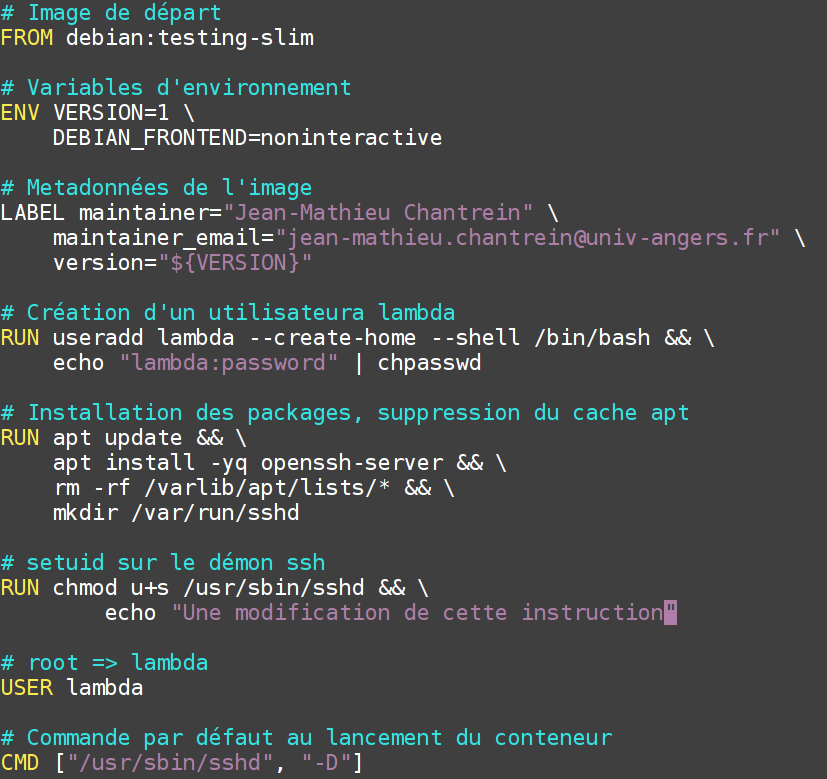
\includegraphics[width=6.4cm]{img/dockerfile_sshd2.png}
			\end{exampleblock}
		\end{frame}
		
		\begin{frame}{La méthode efficace: Dockerfile}
		\vspace{-0.3cm}
			\begin{exampleblock}{Dockerfile serveur ssh: notions de contexte et de cache}
				\small
				\only<1>
				{
					\begin{shell}{}
						\promptsshd docker build . -t sshd
						\tiny
						\verbatiminput{output/build_dockerfile_sshd3.txt} %\end{verbatim}	<-- Ne pas enlever, bug coloration syntaxique
						\small
					\end{shell}
				}
				\only<2>
				{
					\begin{shell}{}
					\tiny
						\verbatiminput{output/build_dockerfile_sshd4.txt}  %\end{verbatim}	<-- Ne pas enlever, bug coloration syntaxique
						\small
						\promptsshd
					\end{shell}
				}
				\only<3>
				{
					\begin{shell}{}
						\promptsshd docker images
						\tiny
						\verbatiminput{output/images_build_sshd_top.txt}
						\small
						\promptsshd docker images -a \# Combien d'images ?
						\tiny
						\verbatiminput{output/images_build_sshd.txt}
						\small
					\end{shell}
				}
				\only<4>
				{
					\vspace{-0.3cm}
					\begin{shell}{}
						\promptsshd docker images -a --filter dangling=true
						\tiny
						\verbatiminput{output/images_build_sshd_dangling.txt}
						\small
						\promptsshd docker rmi 1c1
						\tiny
						\verbatiminput{output/images_build_sshd_rmi.txt}
						\footnotesize
					\end{shell}
					\vspace{-0.3cm}
					\begin{itemize}
						\item Suppression automatique des images non utilisées (i.e.: n'étant parentes d'aucune top level image taguée)
					\end{itemize}
				}
				\normalsize
				\only<5>
				{
					\begin{shell}{}
						\promptsshd docker images -a \# Combien d'images ?
						\tiny
						\verbatiminput{output/images_build_sshd_after_rmi.txt}
						\normalsize
					\end{shell}
					\begin{itemize}
						\item Les images non utilisées ont bel et bien été supprimées
					\end{itemize}
				}
				\only<6>
				{
					\begin{shell}{}
						\promptsshd docker history sshd
						\tiny
						\verbatiminput{output/history_build_sshd.txt} %\end{verbatim}	<-- Ne pas enlever, bug coloration syntaxique
						\normalsize
					\end{shell}
					\begin{itemize}
						\item Les images de taille 0 n'ont pas généré de layer et reposent sur les \textit{layers} des images parentes (on parle de layer vide (empty layer)) 
						\item Pourquoi y a-t-il une différence de 3 jours dans la création des images ?
					\end{itemize}
				}
				\normalsize
				
			\end{exampleblock}
		\end{frame}
		\begin{frame}{La méthode efficace: Dockerfile}
			\only<1-7>
			{
				\begin{block}{Encore quelques informations}
						\begin{itemize}
							\item Il est important de taguer/versionner ses images de production
							\pause	
							\item Les images les plus lourdes devraient être les plus basses (utilisation efficace du mécanisme du cache)
							\pause
							\item Les instructions susceptibles de changer régulièrement devraient se situer dans les couches basses
							\pause
							\item Attention aux directives "update" et "install" lors de l'utilisation du cache
							\pause
							\item Tout changement de contexte (modifications d'un fichier ajouté par ADD ou COPY) entraine une reconstruction des images à partir de la couche affectée
							\pause
							\item Chaque construction (build) d'un Dockerfile génère une \textbf{nouvelle} image (modulo une utilisation totale du cache).
							\pause
							\item Chaque instruction est indépendante (cela n'a pas de sens d'écrire RUN cd /tmp )
						\end{itemize}
				\end{block}
			}
			\vspace{-0.2cm}
			\only<8>
			{
			\begin{shell}{}
			\prompt docker built . -t independant\_instruction
			\verbatiminput{output/independant_instruction.txt}
			\end{shell}
			}
		\end{frame}
		\begin{frame}{Pour info}
			\begin{itemize}
				\item Pour changer de répertoire pour les instructions à suivre (y compris pour d'éventuelles images enfantes) $\Rightarrow$ Utiliser l'instruction WORKDIR
			\end{itemize}
		\end{frame}

\begin{frame}{}
			\begin{exampleblock}{A vous}
				\begin{itemize}
					\item Rédigez un dockerfile permettant de créer une image "mon\_image" à partir d'une ubuntu 16.04
					\item Cette nouvelle image contiendra le paquet inetutils-ping
					\item La commande par défaut doit être ping localhost (instruction CMD)
					\item Testez votre image en instanciant un conteneur
					\item Essayez de surcharger la commande par défaut en la remplaçant par ping qwant.com
				\end{itemize}	
			\end{exampleblock}
\end{frame}

\begin{frame}{}
			\vspace{-0.25cm}
			\begin{exampleblock}{Différence entre les intructions CMD et ENTRYPOINT}
				\begin{itemize}
					\item Construisez l'image du Dockerfile suivant avec docker build . -t ping:
					\verbatiminput{output/cmd_vs_entrypoint.txt} %\end{verbatim}	<-- Ne pas enlever, bug coloration syntaxique
					\item Instanciez cette image sans surcharge avec \textit{docker run ping}
					\item Instanciez cette image en surchargeant avec \textit{docker run ping qwant.com}
				\end{itemize}			
			\end{exampleblock}
			\only<2>
			{
			\begin{block}{}
				\begin{itemize}
					\item ENTRYPOINT permet de se servir d'un conteneur comme d'un exécutable
					\item On peut surcharger ENTRYPOINT avec l'option --entrypoint
					\item On peut modifier les paramètres de l'exécutable définit dans ENTRYPOINT en surchargeant CMD
					\item On peut ajouter des paramètres à ENTRYPOINT qui ne seront pas surchargés par CMD
				\end{itemize}
			\end{block}
			}
\end{frame}


\section{Toujours plus loin}
	\subsection{Travaux pratiques}
		\begin{frame}{Travaux pratiques: de dockerfile à docker swarm en passant par docker compose}
			\begin{exampleblock}{Réaliser un service wordpress conteneurisé}
			 \begin{itemize}
			 	\item Nous changeons de support afin de passer (enfin) à la pratique
			 	\item Merci de vous rendre sur la page web suivante: \url{https://github.com/jmchantrein/formation_docker/blob/master/travaux_pratiques.md}
			 \end{itemize}
			\end{exampleblock}
		\end{frame}


%%%%%%%%
% TODO %
%%%%%%%%
	
%Parler de https://github.com/moncho/dry	
		


%	\subsection{Gestion du réseau}
%	\subsection{Usine logiciel}
%	\subsection{Docker compose}
%	\subsection{Docker swarm}
%		\begin{frame}{Swarm}
%			\begin{block}{Orchestration}
%				\begin{itemize}
%					\item L'orchestration est un mécanisme qui permet de gérer automatiquement la haute disponibilé d'une application sur plusieurs serveurs. 
%					\item En cas d'arret d'un des serveurs, l'orchestrateur permet à l'application d'être toujours accessible.
%					\item Swarm (essaim) est un orchestrateur de conteneur.
%					\item Lorsque swarm est activé sur un cluster de machine, celui-ci est composé d'au moins un leader(manager)
%					\item Les autres hôtes sont appelés les travailleurs (worker)
%					\item C'est depuis l'hôte leader que l'on orchestre les conteneurs.
%					\item Si l'hôte leader qui tombe en panne, soit un autre hôte prend le relais, sinon les workers continue de travailler en roue libre ...
%					\item Le manager maintient l'état de l'essaim et gère les applications conteuneurisé.
%					\item Le worker exécute les applications conteneurisées.
%				\end{itemize}
%			\end{block}
%		\end{frame}

%%%%%%%%%%%%%%%%%%%%%%%%%
% TEMPLATE EXAMPLE      %
%%%%%%%%%%%%%%%%%%%%%%%%%
%		\begin{frame}
%			\begin{exampleblock}{Template}
%				\begin{minipage}[T]{.7\textwidth}
%					\begin{shell}{}
%					\tiny
%					\only<1>{\begin{text}
%							\prompt docker run hello-world \\
%							Unable to find image 'hello-world:latest' locally\\
%							latest: Pulling from library/hello-world\\
%							78445dd45222: Downloading [===============> \ \ \ \ \ \ \ \ \ \ \ \ \ \ ] \\
%						\end{text}
%					}
%					\only<2>{\begin{text}
%							\prompt docker run hello-world \\
%							Unable to find image 'hello-world:latest' locally\\
%							latest: Pulling from library/hello-world\\
%							78445dd45222: Extracting \ \ \ [=========> \ \ \ \ \ \ \ \ \ \ \ \ \ \ \ \ \ \ \ \ \ \ \ \ \ \ \ ] \\
%						\end{text}
%					}
%					\only<3>{\begin{text}
%							\prompt docker run hello-world \\
%							Unable to find image 'hello-world:latest' locally\\
%							latest: Pulling from library/hello-world\\
%							78445dd45222: Pull complete \\
%							Digest: sha256:c5515758d4c5e1e838e9cd307f6c6a0d620b5e07e6f927b07d05f6d12a1ac8d7\\
%							Status: Downloaded newer image for hello-world:latest\\
%							...
%						\end{text}
%					}
%					\end{shell}
%				\end{minipage}%
%				\begin{minipage}[T]{.3\textwidth}
%						\begin{enumerate}
%							\item Téléchargement de l'image
%							\item<2-> Désarchivage de l'image
%							  
%						\end{enumerate}
%				\end{minipage}
%			\end{exampleblock}
%		\end{frame}

%Conteneurisation orientée système d'exploitation --> full conteneurisation
%\section{LXC}
%	\subsection{Introduction}
%	\subsection{LXD/LXC}
%	\subsection{Proxmox LXC}

%Conteneurisation orientée calcul scientifique
%\section{Singularity}

%\begin{frame}{Introduction}
%	\begin{block}{Qu'est-ce que la conteneurisation ?}
%		\begin{itemize}
%			\item Il ne s'agit pas de 
%			\item<2> Deuxièmement
%		\end{itemize}
%	\end{block}
%\end{frame}




\end{document}
